\subsection{Guarded Acquisition and Wireless Confirmations}
\label{app:v37-study}
We evaluate the audited guarded controller separately from the earlier studies. We freeze the implementation, case labels, random seeds, comparisons, and analysis before generating the final outcomes. The primary variant retains the fresh acquisition rule and uses audited history only in verification and promise calculations. We also evaluate history-guided ordering, balanced ordering, guarded fresh acquisition, and five unchanged earlier baselines. All methods retain the original report prices, acquisition durations, instrument caps, and return-verifier coefficient.

\subsubsection{Protocol and Primary Comparison}
The single-goal confirmation contains 21 declared case labels: the nine original envelope/drift settings and twelve extension labels that include feasibility, violation, bottleneck, boundary, and response-ambiguity cases. Three extension parameter tuples duplicate original tuples; they use independent tapes, retain their declared labels, and are also reported separately. Each label receives 32 new tapes, paired across two budgets and nine methods, giving 1344 decisions per method. An earlier eight-tape-per-label development study remains separate. No case or method is removed after outcomes are observed.

We prespecify a minimum mean-cost reduction of $2\%$ and a completion noninferiority tolerance of one percentage point. We resample tapes within each declared case, preserving both budgets and method pairing. The paired percentile bootstrap intervals are descriptive; they are not distribution-free finite-sample confidence guarantees. The primary must have a cost-reduction lower endpoint above $2\%$ and a completion-difference lower endpoint above $-1$ percentage point to pass both criteria. All-attempt costs include unresolved decisions.

\begin{table}[t]
\caption{Final Single-Goal Comparisons: 1344 Decisions per Method}
\label{tab:v37-methods}
\centering\footnotesize
\begin{tabular}{lrrr}
\toprule
Method & Mean cost & Correct & Unresolved\\
\midrule
Fresh proportional & 3021.64 & 1128 & 216\\
Fresh repaired & 2962.29 & 1128 & 216\\
Fresh slack & 2947.11 & 1128 & 216\\
Guarded fresh & 2996.73 & 1129 & 215\\
Audited, history-guided actions & 2994.15 & 1128 & 216\\
Audited, balanced actions & 3015.73 & 1129 & 215\\
Audited, fixed fresh actions & 2992.60 & 1129 & 215\\
Earlier audited repaired & 3130.14 & 1128 & 216\\
Earlier sufficient controller & 3130.14 & 1128 & 216\\
\bottomrule
\end{tabular}
\end{table}

Table~\ref{tab:v37-methods} retains every comparator. The primary reduces mean cost relative to guarded fresh by $0.138\%$, with paired interval $[0.082\%,0.201\%]$, and has identical completion outcomes. It fails the $2\%$ cost criterion. All 1344 paired primary paths obey the single-goal cost and duration ordering; only 57 obtain strict cost savings, with a maximum saving of 304 units. This replay check supports implementation fidelity; Proposition~\ref{prop:v37-fixed-actions} supplies the pathwise argument.

For the original-grid subset, both methods complete 575 of 576 decisions, at mean costs 1924.59 and 1931.64, respectively. For the extension subset, both complete 554 of 768, at 3793.61 and 3795.55. The 192 boundary or low-margin decisions remain unresolved under both methods. Lower expenditure on an unresolved attempt alone is not an efficiency gain.

The primary costs $1.023\%$ more than unguarded fresh repaired, with paired interval $[0.815\%,1.233\%]$, and completes one additional decision. Its $4.394\%$ lower cost than the earlier audited controllers includes a different initial audit schedule and does not isolate planning efficiency. History-guided actions lose one completion relative to guarded fresh; the fixed-action preservation argument does not apply to that variant. No incorrect return is observed, but empirical absence of errors does not replace the validity theorem.

\begin{figure}[t]
\centering
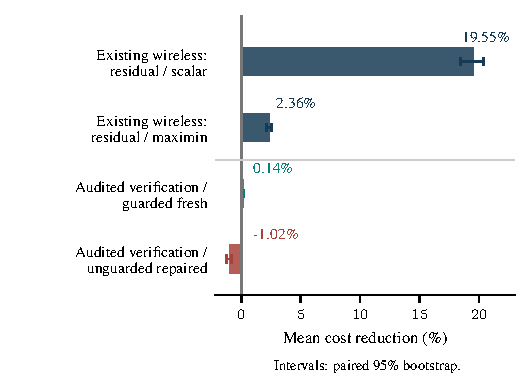
\includegraphics[width=\columnwidth]{figures/v37_cost_comparisons.pdf}
\caption{Separate frozen comparisons. The upper rows confirm existing nine-configuration wireless controllers on 32 complete four-goal sequences; the lower rows evaluate the new audited-verification variant on 1344 two-instrument decisions. Positive values denote lower all-attempt cost. The last comparison has one additional completion for the audited variant. Intervals preserve the paired experimental units; the populations and controller interfaces are not pooled.}
\label{fig:v37-costs}
\end{figure}

\subsubsection{Promise Availability and Reservation Quality}
The primary issues 500 promises among 1344 initially unresolved decisions ($37.20\%$), compared with 484 ($36.01\%$) for guarded fresh. Every primary promise is met by an actual correct return at or before its first advertised endpoint. A separate analysis also reconstructs the frozen certificate at its hypothetical full endpoint. That diagnostic may use reports the actual controller did not acquire; those reports never enter acquisition decisions or measured expenditure.

The earlier sufficient controller issues 39 plans among 1152 decisions unresolved after its larger initial audit ($3.39\%$). Its joint planning-failure allowance is $0.105$, compared with the new promise bound of $0.05$; its initial measurements and planning opportunities also differ. This comparison is diagnostic and does not replace the earlier recorded $37/1312$ result or establish an isolated causal effect of the new planner.

For the 500 primary promised decisions, mean cost already spent at issuance is 874.13 units. Mean advertised additional cost is 7352.62, whereas mean actual additional cost is 347.89. Mean advertised total cost is 8226.76, compared with actual total cost 1222.03; the median ratio of advertised to actual total cost is 6.75. Figure~\ref{fig:v37-promises} displays the additional costs. These post hoc descriptive diagnostics expose loose reservations; the controller is not retuned after they are calculated. Issuance frequency does not establish tight or near-optimal completion planning. The theorem controls the joint event of issuance and failure, not uniform conditional reliability among issued promises.

\begin{figure}[t]
\centering
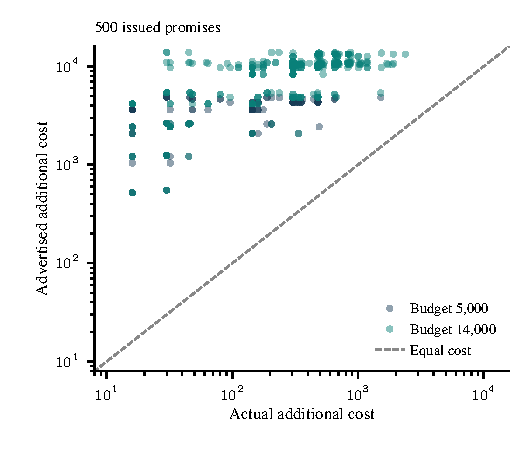
\includegraphics[width=\columnwidth]{figures/v37_promise_reservations.pdf}
\caption{Advertised and actual additional acquisition cost for the primary controller's 500 issued promises. Both axes are logarithmic. All promises complete in these trials, but reservations are conservative. These selected-promise diagnostics complement the all-attempt comparison in Table~\ref{tab:v37-methods}; they do not establish a conditional probability guarantee.}
\label{fig:v37-promises}
\end{figure}

\subsubsection{Shared-Epoch Goal Changes}
We separately test 32 further tapes per original-grid label under both budgets and the four threshold pairs $(5.8,4.8)$, $(2.9,1.9)$, $(1.4,0.9)$, and $(5.8,4.8)$. The four guarded methods share absolute count checkpoints, retain acquired evidence, and never reset physical quotas or validity risks during a sequence. We allocate future promise risk $0.03/4$ per possible first promise.

The primary and guarded fresh each complete all four goals in 563 of 576 budget-specific epochs. Their mean epoch costs are 2196.56 and 2210.54, a reduction of $0.633\%$ with paired interval $[0.319\%,1.022\%]$. The primary's mean additional costs across the goals are 144.33, 1873.44, 178.78, and zero; the corresponding fresh costs are 144.33, 1887.74, 178.47, and zero. The third goal can cost more under the primary, consistent with the absence of a sequence-wide pathwise comparison. Every method resolves the final relaxed goal without new reports, illustrating shared-epoch evidence reuse rather than a gain unique to historical auditing. History-guided actions cost 2184.72 on average and also complete 563 epochs; balanced ordering costs 2379.14 and completes 562. We retain both outcomes.

\subsubsection{Wireless Confirmation and Replay Checks}
We also freeze 32 new four-goal sequences for the existing complete nine-configuration wireless model. We preserve the original $24\to12.6\to9.5\to24$-ms goals, report family, per-instrument caps, historical support, and global 20000-unit acquisition-time window. That window is not an additional cost cap. Two matched-interface comparisons isolate existing residual versus scalar allocation and existing residual versus alternative-information maximin. They do not apply the new two-instrument controller to nine configurations.

All 512 decisions complete correctly. Residual versus scalar allocation has mean sequence costs 2661.84 versus 3308.72, a $19.55\%$ reduction with paired interval $[18.46\%,20.40\%]$. Under the stronger common interface, residual versus alternative-information maximin costs 2739.90 versus 2806.12, a $2.36\%$ reduction with interval $[2.13\%,2.57\%]$. Both 24-ms goals require no new reports throughout; the 12.6-ms goal needs none in 22 of 32 sequences. These are controlled confirmations of the existing methods. The earlier $93.1\%$ stopping result has a different population and comparator and remains separate.

Independent replay verifies every recorded decision, acquisition prefix, resource ledger, and issued promise in both new studies. All checks pass; the audits reconstruct observations without importing the candidate controller or verifier for their core calculations. Frozen protocols, source snapshots, complete results, and replay scripts accompany the paper. These checks assess implementation fidelity under the declared model; zero observed errors do not establish rare-event reliability or physical deployment performance.
